%\chapter{Image Style Transfer}\chlbl{image_style_transfer}
%In the field of image style transfer\sidecite{Gatys_Ecker_Bethge_2015}, such correlations are used to generate images.
%An image is created based on two images, one image providing the content (i.e. the ``content-image'') and the other image providing the style (i.e. the ``style-image'').
%To generate the content of the image, a random image can be fed into the model and a simple distance-based loss function such as the Euclidean norm can be used to calculate the difference between the model output and the content-image.
%Over time, the model would learn to output the content-image.
%However, only the content from the content-image and not its style is needed.
%A solution to this problem is using Convolutional feature maps\sidenote{a convolutional layer can have multiple filters (i.e. channels), each filter produces a convolutional feature map} as they capture spatial information of an image well, while containing only little style information.
%Therefore, the distance loss is not calculated between the content-image and the model output but between the feature maps of the content-image and the output image.

%The second task is to transfer the style from the style-image to the model output.
%The style of an image can be described by correlations across the different feature maps.
%This information about the image style can be calculated with a Gram matrix.
%A Gram matrix is the dot product\sidenote{the dot product between two vectors can be seen as similarity metric; it gets bigger if two vectors are more similar} of the flattened feature vectors from a convolutional feature map (i.e. the dot product between all channels of a convolutional layer's output).
%For example, a convolutional layer could have multiple channels. The first channel could have a high activation for black and white stripes in horizontal direction while the second channel could have a high activation for black and white stripes in vertical direction. If both channels activate together for the same input and thus have a high correlation, there is a high possibility that the image might contain the style of a chessboard (i.e. black and white checkered). A third channel, for example, could have a high activation for eyes. If this channel has a low correlation with the first channel but a high correlation with the second channel (i.e. black and white stripes in vertical direction), the input image might contain the face of a zebra and thus capture a ``zebra-style''.
%Similar to the content-transfer, a distance loss such as the Euclidean distance can be used to compare the Gram matrices of the style-image and the output-image.
%Thus, it is compared if the output-image has the same style as the style-image.

%In summary, the content is transferred by comparing entire convolutional layer output and the style by comparing the correlations between the feature maps of a convolutional layer output (i.e. by comparing gram matrices).

%\pagebreak
%\chapter{Design Decisions}\chlbl{design_decisions}
%There exists a variety of possibilities how self-organization of the network architecture can be implemented.
%However, this thesis is of course limited in time and resources an thus not all of them can be investigated.
%Therefore, a promising direction of research had to be defined at the beginning and followed afterwards.

%As a constraint it was defined that (i) a network without dynamics is developed and (ii) self-organization takes place across multiple layers.
%A network without dynamics is used because Deep Learning works very well for pattern recognition and the data analyzed by the computer is mostly static.
%Dynamic networks usually have poorer performance and use special algorithms to convert static data such as images into dynamic time-related signals (c.f. Section \secref{self_org_spiking}).
%Applying self-organization across multiple layers rather than just adding lateral connections in one layer is preferred as this allows the network to form more complex structures and thus to use the whole potential of self-organisation.

%This thesis is strongly inspired by the paper ``Natural Intelligence'' \sidecite{von_der_Malsburg_Stadelmann_Grewe_2022} (c.f. Section \secref{natural_intelligence}).
%The most relevant findings in this work are:

%\begin{itemize}
%  \item The brain is highly structured
%  \item Self-organization is the most promising approach to achieve natural intelligence. It loops between activity and connectivity
%  \item Self-organization forms net-fragments, one neuron can be part of multiple fragments
%  \begin{itemize}
%    \item An object can be represented by multiple net-fragments
%    \item A hierarchy of features can be represented by nested net-fragments
%  \end{itemize}
%  \item The self-organizing process has to start from an already established coarse structure
%  \item There exists many alternative pathways in the network
%\end{itemize}

%However, it is unclear how these findings and hypotheses from the field of neuroscience can be implemented in an algorithm.
%To create a self-organizing neural network, the following mechanisms are particularly relevant: The design of the initial architecture, the allowed architecture modifications (removing and adding neurons and/or connections), the type of neurons, and the definition of the learning algorithm.
%These aspects are discussed hereafter.

%\begin{description}
%   \item[Design of initial architecture] The initial architecture should exhibit a good inductive bias from the start so that the network can learn (something meaningful). Current approaches also start from much bigger architectures and reduce their size by up to a thirty-fold \sidecite{Pedersen_Risi_2021} (c.f. Section \secref{self_org_related}) or grow the architecture from a single neuron \sidecite{Raghavan2019NeuralNG} (c.f. Section \secref{self_org_spiking}) by using self-organisation.
%   \item[Architecture modifications] The architecture can be modified in several ways. For example, from a more global perspective, the network can grow, shrink, split into sub-networks\sidenote{this is related to ensemble approaches TODO: add source}, or multiple sub-networks can re-organize into one network. From a local perspective, connections can be created or removed within the same layer (lateral connections) or between subsequent layer. Moreover, connections can be used to skip on or several layers (residual connections), or connections can be recurrent to a previous layer. Furthermore, besides modifying single connections and neurons, complete blocks of neurons can be added or removed. This includes for example layers, mathematical functions like pooling operations, or pre-defined modules consisting of several layers.
%   \item[Type of neurons] As described above, no dynamic (i.e. spiking) neurons are employed. The classical neurons multiply the input \(\boldsymbol{x}\) by a weight vector \(\boldsymbol{w}\), add a bias \(\boldsymbol{b}\) and calculate the output with a non-linear activation of this sum (c.f. Section \secref{ann}). However, recent architectures replace such classical neurons with more complex units. For example, Kirsch and Schmidhuber \sidecite{kirsch2021meta} (c.f. Section \secref{self_org_related}) use tiny RNNs with shared parameters as neurons. Such neurons are able to learn learning algorithms which are equivalent to back-propagation.
%   \item[Learning algorithm] ... (see learning to learn or Hebbian based on input covarinace or learning based on target label (e.g. enforce some distinction in neurons covariance matrix depending on label))
%\end{description}


\pagebreak
\chapter{Experiments Hebbian Learning}\chlbl{exp_hebb_learning}
I used different variants of Hebbian Learning with the goal of generating good latent representations of visual scenes.
However, all preliminary experiments with different implementations were not promising.
In my experiments, classical Hebbian learning (as described in Equation \eqref{hebb_1}) led to symmetric weights, which in turn led to poor representations.
This symmetry could be broken by using the ABCD-Hebbian learning rule \sidecite{Niv_Joel_Meilijson_Ruppin_2001}.
The ABCD learning rule calculates the weight update \(\Delta w_{ij}\) from neuron \(i\) to neuron \(j\) based on the pre-synaptic activity \(r_i\) of neuron \(i\) and post-synaptic activity \(r_j\) of neuron \(j\) as follows:

\begin{equation}\eqlbl{hebb_abcd}
	\Delta w_{ij} = \eta_w \cdot (A_wr_ir_j+B_wr_i+C_wr_j+D_w)
\end{equation}

where \(\eta_w\) is a weight-specific learning rate, and \(A_w\) is a correlation coefficient, \(B_w\) is a presynaptic coefficient, \(C_w\) is a postsynaptic coefficient, and \(D_w\) is a bias coefficient.
The bias coefficient \(D_w\) can be interpreted as an individual inhibitory or excitatory bias of each connection in the network.
Similar to Najarro and Risi \sidecite{NEURIPS2020_ee23e7ad}, the coefficient were learnt through an evolution strategy \sidecite{Salimans_Ho_Chen_Sidor_Sutskever_2017}.
However, this method does not scale for large networks with many parameters and did not achieve the desired performance in my experiments.

Of course, it cannot be concluded from these experiments that Hebbian Learning cannot be used to learn networks for extracting good representation from visual scenes.
However, it was found that it is not trivial and that just applying the Hebbian learning rule is not sufficient, especially if the network has a structure of modern Deep Learning architectures with many parameters.

However, in further preliminary experiments it was found that Hebbian Learning has interesting properties for pruning.
A good performing CNN was created and trained on MNIST with backpropagation.
The network consists of two convolutional layers, followed by a pooling layer and three linear layers.
The first convolutional layer increases the number of channels from \([\text{width} \times \text{height} \times \text{n\_channels}]\) to \([\text{width} \times \text{height} \times 32]\).
The second convolutional layer further increases the number of channels to \([\text{width} \times \text{height} \times 64]\).
The subsequent max. pooling layer decreases the size to \([\text{width}/2 \times \text{height}/2 \times 64]\).
The activation map is then flatten and fed into 3 fully connected layers with an output size of \(1024\), \(128\), and \(10\) respectively.
Between each layer, ReLU activtions are employed.
The network is visualized in Figure \figref{hebb_pruning}.

\begin{figure}[h]
    \centering
    \resizebox{0.99\textwidth}{!}
{
	\begin{tikzpicture}
		\tikzstyle{connection}=[ultra thick,every node/.style={sloped,allow upside down},draw=\edgecolor,opacity=0.7]
\tikzstyle{copyconnection}=[ultra thick,every node/.style={sloped,allow upside down},draw={rgb:blue,4;red,1;green,1;black,3},opacity=0.7]


\pic[shift={(0,0,0)}] at (0,0,0) 
    {Box={
        name=conv1,
        caption=Conv + ReLU,
        xlabel={{1, }},
        zlabel=32,
        fill=\ConvColor,
        height=16,
        width=4,
        depth=16
        }
    };


\pic[shift={(3,0,0)}] at (0,0,0) 
    {Box={
        name=conv2,
        caption=Conv + ReLU,
        xlabel={{32, }},
        zlabel=64,
        fill=\ConvColor,
        height=16,
        width=8,
        depth=16
        }
    };


\draw [connection]  (conv1-east)    -- node {\midarrow} (conv2-west);


\pic[shift={ (0,0,0) }] at (conv2-east) 
    {Box={
        name=pool1,
        caption= ,
        fill=\PoolColor,
        opacity=0.5,
        height=8,
        width=1,
        depth=8
        }
    };


\pic[shift={(4,0,0)}] at (pool1-east) 
    {Box={
        name=fcn1,
        caption=Hebb. Pruning + ReLU,
        xlabel={{" ","dummy"}},
        zlabel=1024,
        fill=\SoftmaxColor,
        opacity=0.8,
        height=3,
        width=3,
        depth=100
        }
    };


\draw [connection]  (pool1-east)    -- node {\midarrow} (fcn1-west);


\pic[shift={(2,0,0)}] at (fcn1-east) 
    {Box={
        name=fcn2,
        caption=Hebb. Pruning + ReLU,
        xlabel={{" ","dummy"}},
        zlabel=128,
        fill=\SoftmaxColor,
        opacity=0.8,
        height=3,
        width=3,
        depth=50
        }
    };


\draw [connection]  (fcn1-east)    -- node {\midarrow} (fcn2-west);


\pic[shift={(2,0,0)}] at (fcn2-east) 
    {Box={
        name=fcn3,
        caption=FCN + Softmax,
        xlabel={{" ","dummy"}},
        zlabel=10,
        fill=\SoftmaxColor,
        opacity=0.8,
        height=3,
        width=3,
        depth=25
        }
    };


\draw [connection]  (fcn2-east)    -- node {\midarrow} (fcn3-west);

\end{tikzpicture}
}
    \caption[Hebbian Pruning Network]{The network architecture used to perform Hebbian-based weight pruning.}
    \figlbl{hebb_pruning}
\end{figure}

The image classification model is trained with backpropagation to minimize the negative log likelihood (NLL) loss.
Adam \sidecite{Kingma_Ba_2017} is used as optimization algorithm with a mini-batch size of \(32\) a learning rate of \(5\cdot 10^{-4}\).
As soon as the loss reaches a plateau, the learning rate is reduced to \(1\cdot 10^{-4}\).

After the model is trained, the first two fully connected layers within the network are pruned with Hebbian learning based methods.
The convolutional layers cannot be pruned because such layers employ a convolutional function that impedes calculating the correlation between an input and an output neuron.
The last layer, on the other hand, cannot be pruned as it corresponds to the number of classes.

The \emph{first} Hebbian based method proposed pushes the weights between neuron \(i\) and neuron \(j\) towards \(0\) if \(i\) and \(j\) have a low correlation within a mini-batch.
First, a mini-batch is sampled.
Afterwards, the correlation between \(i\) and \(j\) is calculated for each sample.
if the correlation is below \(0.02\) for at least \(20\%\) of the samples (i.e. \(7\) samples or more for a mini-batch size of \(32\)), the weight is updated as follows:
\begin{equation}\eqlbl{hebb_towards_0}
	\Delta w_{ij} = - \eta_H \cdot w_{ij}
\end{equation}

where \(\eta_H\) is the Hebbian learning rate set to \(1\cdot 10^{-5}\).

The \emph{second} Hebbian based method proposed pushes some of the weights exactly to \(0\) while all other weights remain the same.
During an epoch, the correlation between neurons \(i\) and \(j\) is measured for each weight \(w_{ij}\).
Afterwards, the weights with the lowest correlations are set to \(0\).
How many weights are set to \(0\) is a hyper-parameter that has to be specified in advance.

For both methods, the model is pre-trained and pruned on the MNIST dataset \cite{MNIST} and evaluated on the MNIST as well as on the MNIST-C\sidenote{MNIST-C is a corrupted version of MNIST and well suited to measure model robustness} dataset \cite{Mu_Gilmer_2019}.
The \emph{first} Hebbian based method can improve the results even after backpropagation as shown in Table \tabref{nll_hebb_pruning}.

\begin{table}[h] 
    \tablbl{nll_hebb_pruning}
    \centering
	 \begin{tabular}{|l c c|} 
    	\hline
    	 & NLL-Loss & NLL-Loss \\
        Dataset & without Hebbian Updates & with Hebbian Updates\\
        \hline
        MNIST & \(0.05314\) & \(0.03386\) \\
        MNIST-C & \(0.6013\) & \(0.4766\) \\
        \hline
    	 &Accuracy & Accuracy \\
        Dataset & without Hebbian Updates & with Hebbian Updates\\
        \hline
        MNIST & \(98.94\%\) & \(98.97\%\) \\
        MNIST-C & \(88.74\%\) & \(89.94\%\) \\
        \hline
    \end{tabular}
    \caption[NLL Loss of Hebbian Pruning Network]{NLL loss of the model before and after the \emph{first} Hebbian-based pruning method.}
\end{table}

The NLL-loss on the MNIST test dataset decreases from \(0.05314\) to \(0.03386\), while the loss on MNIST-C test dataset decreases from \(0.6013\) to \(0.4766\) after applying the \emph{first} Hebbian based method.
However, in terms of accuracy the improvements are marginal.
Furthermore, it has to be considered that this is only a preliminary experiment and this method certainly offers various potential for improvement.
This experiments indicates that Hebbian in combination with back-propagation could lead to better or more robust representations because the Hebbian updates improved performance on both datasets.

The \emph{second} Hebbian based method sets weights between neurons with a low correlation to \(0\).
The network trained with back-propagation has an accuracy of \(98.94\%\) on MNIST.
By setting up to \(40\%\) of the weights to \(0\), the accuracy remains above \(>98\%\).
Setting weights to \(0\) can make the network smaller and more efficient \sidecite{Liang_Glossner_Wang_Shi_Zhang_2021}.
Furthermore, it leads to sparse representations that can improve robustness.
Figure \figref{hebb_prune} visualizes the loss of the \emph{second} Hebbian based method for different ratios of kept weights.
Furthermore, the correlation based method is compared to randomly setting the same fraction of weights to \(0\).

\begin{figure}[h]
    \centering
    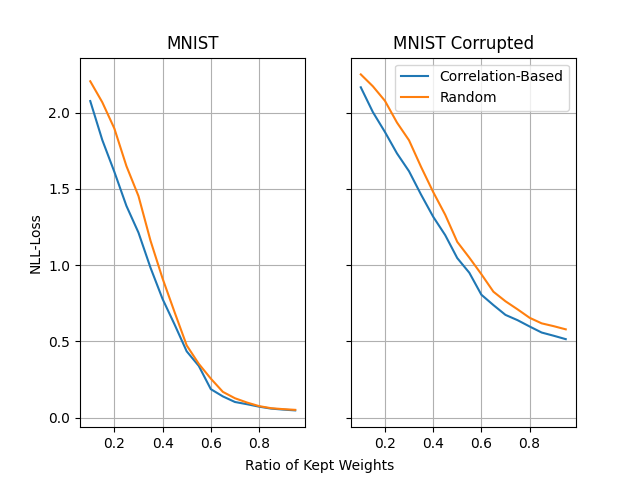
\includegraphics[width=0.99\textwidth]{loss_hebb_pruning}
    \caption[NLL Loss of Hebbian Pruning]{The NLL loss of the \emph{second} Hebbian based pruning method compared to removing random weights. The y axis shows the loss while the x axis shos the ratio of weights kept. }
    \figlbl{hebb_prune}
\end{figure}

It can be observed that the performance is better when weights between neurons with low correlation are set to \(0\) than if random weights are set to \(0\).


\pagebreak
\chapter{Net-Fragments and Deep Learning}\chlbl{net_fragments}
In this chapter, it is examined how representations of typical deep learning architectures look like.
Especially net fragments are of interest, i.e. (groups of) neurons that represent certain features of objects.
Net-fragments are discussed in Section \secref*{neuro_concepts_net_fragments}.
There, it is described that the interpretation of net-fragments in this thesis relies on two principles:

\begin{itemize}
	\item The latent representations should be read out from multiple layers and not from a single layer
	\item To obtain meaningful activations, the activation maps should be sparse and diverse
\end{itemize}


%According to \sidecite{von_der_Malsburg_Stadelmann_Grewe_2022}, net fragments are a compositional data structure (c.f. Section \secref*{natural_intelligence}).
%In architectures without recurrent connections, a composition of neurons is built up hierarchically over several layers.
%Thus, an object is not represented by the activations of a single layer but by the activations of multiple layers (c.f. Section \secref*{neuro_concepts_net_fragments}).
%Furthermore, groups of neurons represent certain features, and an object is composed of a multitude of such neuron groups (i.e. has many features).

% TODO schreiben, dass NN nur letztes Layer auslesen -> dieses Prinzip verletzt, zweites Prinzip ist das Neuronen spezifische Features repräsentieren -> das wird hier untersucht
%Typical deep learning architectures for vision tasks sequentially process the input, i.e. the output from one layer is used as input from the next layer.
%In the last layer\sidenote{or in some special cases such as autoencoders in a defined intermediate layer}, the representations describing the objects in the image are retrieved and used for a down-stream task such as image classification.
%Thus, object representations stem from one single layer.
%This process violates the biological principle that an object is represented by groups of neurons that span over several layers.
%However, even if deep-learning architectures use only one layer to represent objects, they work very well due to the increasing complexity of features within a neural network; deep learning architectures for image processing, especially CNNs, build a hierarchy of features where the first layers extract low-level features that are combined into more complex features in the later layers. The last layer thus represents objects but neglects the details.

The first principle is violated by most deep learning architectures as the latent representations are read out from a single layer and subsequently used for a downstream task.
Since this first principle is violated by deep learning architectures by design, this chapter focuses mainly on the second principle. Specifically, it investigates whether specific neuron groups can be assigned to specific features (i.e. represent net-fragments). 
If this would be the case, specific features would be expected to trigger the activation of a group of neurons when they are present and that the same neurons would be inactive when this feature is not present. Thus, different neurons should be active for different objects.
It is important to note that this mainly improves robustness and interpretability. Sparsity and diversity is not necessary, for example, to achieve high classification accuracy.

Deep Learning architectures usually consist of several layers with millions of neurons, leading to millions of activations \cite{Szegedy_Liu_Jia_Sermanet_Reed_Anguelov_Erhan_Vanhoucke_Rabinovich_2014, He_Zhang_Ren_Sun_2016, Ronneberger_Fischer_Brox_2015, He_Gkioxari_Dollar_Girshick_2017, Liu_Anguelov_Erhan_Szegedy_Reed_Fu_Berg_2016, Redmon_Divvala_Girshick_Farhadi_2016}.
Thus, the input data is processed in a complex way, which makes the analysis of activations difficult.
To simplify the analysis of network activations, a novel straightforward classification dataset is proposed;
The dataset consists of $10$ images as shown in Figure \figref*{pre_study_dataset}.
Each image has a size of $9\times9$ pixels and depicts a number between $0$ and $9$.
The images have only one channel and contain binary values (i.e. pixels are either set to $0$ or $1$).
Small networks are sufficient to analyze these images and this dataset thus leads to less network activations what simplifies the search for net fragments.

\begin{figure}[h]
    \centering
    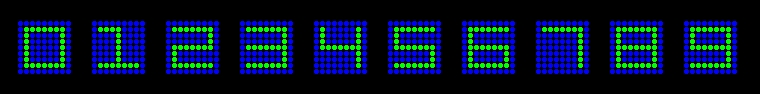
\includegraphics[width=0.99\textwidth]{pre_study_dataset}
    \caption[Straight Line Digits Dataset]{A novel dataset created to investigate the properties of modern deep learning architectures. The dataset consists of images of the numbers $0-9$, each image has a size of $9\times9$ pixels. The blue dots represent pixels with the value $0$, green dots represent pixels with the value $1$.}
    \figlbl{pre_study_dataset}
\end{figure}

Even in this small data set, there exist various features and consequently a multitude of network fragments.
A very intuitive way for us humans to construct features on this data set is to interpret each line as a feature.
For example, the dataset could be explained by $9$ basic lines, that can be composed to $10$ different digits.
Thus, a low-level net fragment could represent such a basic line and be composed to higher-level net fragments such as digits.
Figure \figref*{pre_study_components} visualizes such an intuitive composition (basic lines on the left, digits on the right).

\begin{figure}[h]
    \centering
    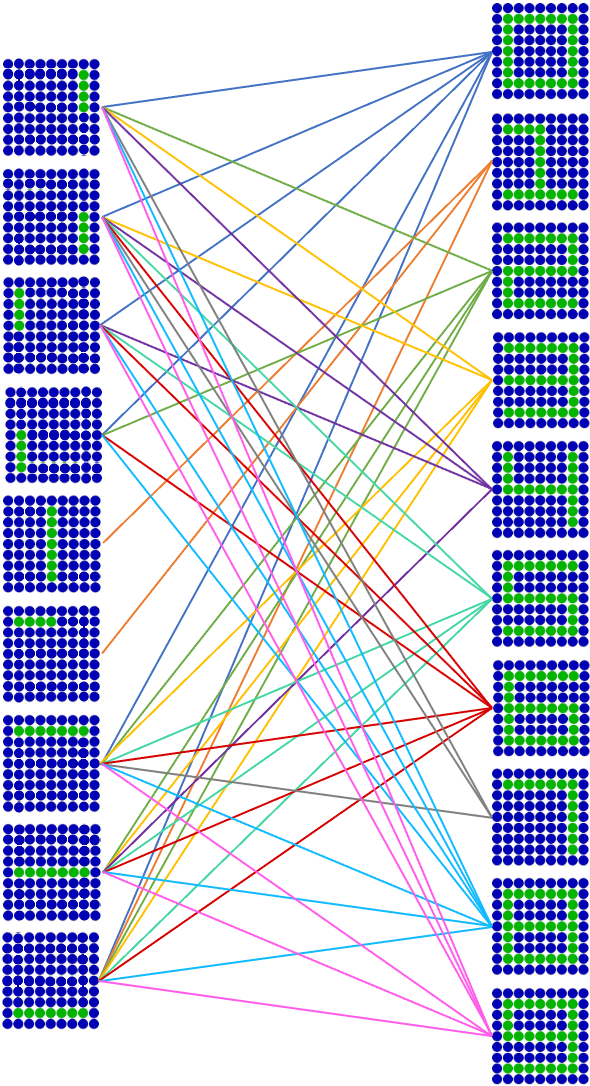
\includegraphics[width=0.99\textwidth]{pre_study_components}
    \caption[Line Types in Straight Line Digits Dataset]{A visualisation of all the lines (left) needed to compose the digits in the data set (right). The coloured lines in-between illustrate the relationship between the lines and the digits.}
    \figlbl{pre_study_components}
\end{figure}

Thereby, each low-level fragment can be part of one or multiple digits.
The composition can either take place across one or multiple layers.
The visualization in Figure \figref*{pre_study_components} can be interpreted as a composition across one layer, i.e. the low-level fragments are combined to high-level fragments within one step.

The composition can also take place across multiple layers. 
An exemplary composition of net fragments of the number $9$ across $4$ subsequent layers is shown in Figure \figref*{pre_study_composition}.
In this example, it is demonstrated that a fragment representing a digit can be composed of other fragments that also represent digits.


\begin{figure}[h]
    \centering
    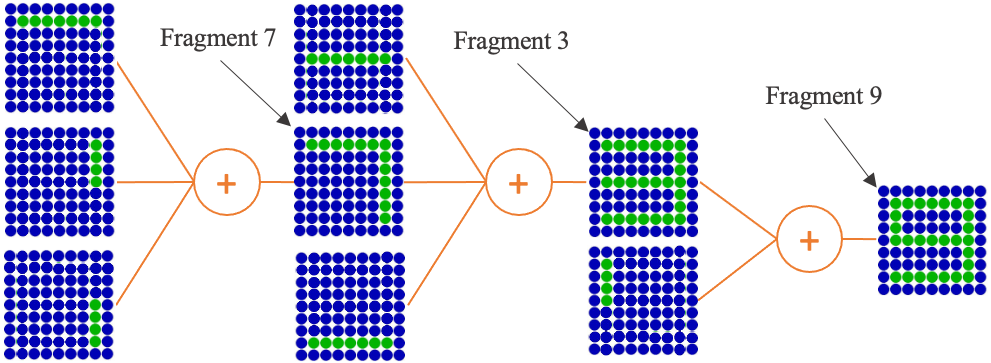
\includegraphics[width=0.99\textwidth]{pre_study_composition}
    \caption[Sample Net Fragment Composition]{A sample composition of the net fragment that could represent the digit $9$.}
    \figlbl{pre_study_composition}
\end{figure}

However, this explanatory example has to be understood as an intuitive way how humans would build net fragments.
Actual net fragments do not necessarily have to be a composition of lines but can be a composition of multiple pixels without semantic.
In fact, it can be expected that neural networks come up with their own features that look totally different than the example used above for explaining net fragments.
Regardless of what these net fragments represent, the network should have certain characteristics;
If a neuron or a group of neurons are part of a net fragment that represents a feature in the input, then these neuron(s) should be strongly active if the feature is present and not or only very weakly active if the feature is not present.
This leads to a sparse activation map and net fragments should only be active for digits with specific characteristics.
Thus, different neurons should be active depending on the digit.

Digits with common characteristics should have some overlapping network activities;
For example, the $7$ is contained in the $3$, the $3$ is contained in the $9$ and the $9$ is contained in the $8$.
Therefore, these digits should have some common network activations.
The $1$, on the other hand, has nothing in common with the $4$, thus these digits should have no overlapping activations.
In the following, networks are trained and their activations are examined for such properties.

Two types of models are trained on this dataset, namely a classification network (supervised) and autoencoder networks (unsupervised).
The goal of the classification task is to predict the number (labels $0-9$) that is shown in the image (c.f. Section \secref*{train_cnns}).
This task is neither for humans nor deep learning architectures challenging.
Usually, the last layer of an image classification architecture has exactly as many neurons as there are classes to predict.
Each neuron corresponds to a class, and the neuron with the highest activity (i.e. the most active neuron) is eventually used to predict the image-level label.
Such architectures thus have the design constraint that the last layer of neurons must represent distinct classes.
Therefore, each neuron in the last layer can be interpreted as a representation of a class-object.
Since the last layer of a classification network represents entire classes, such architectures seem to be well suited to investigate whether the preceding layers represent object features (i.e. net fragments) that are composed by the last layer.

A classification network relies on labels.
An autoencoder, on the other hand, works unsupervised and reconstructs the input data from a lower dimensional embedding space (c.f. section \secref*{visual_rep_learning}).
Thus, the autoencoder generates representations that contain not only the class information but the entire image information.
Consequently, the embedding activations of autoencoders are also examined in the embedding space.
In addition, the autoencoder offers the possibility to constrain the embedding space so that net fragments are more strongly encouraged.



\section{Classification}\seclbl{pre_study_classification}

\subsection{Methods}\seclbl{pre_study_classification_methods}
To investigate the emergence of net fragments in classification networks, different architectures are trained.
The model's parameters are optimised by minimising the cross-entropy loss with the Adam optimizer \sidecite{Kingma2015AdamAM} so that the models learn to predict the corresponding class of the images shown in Figure \figref*{pre_study_dataset}.
The learning rate is $5 \cdot 10^{-4}$, the mini-batch size is $32$ samples and the model is trained for a total of $10$ epochs.

The models used have different feature extractors consisting of either convolutional (Conv.) layers (models no. $1$-$8$, no. $11$) or fully connected (FC) layers (models no. $10$) as shown in Table \tabref*{pre_study_models}.
Model no. $9$ has no feature extractor as the input images are so simple that they can be considered as features by themself, model no. $10$ uses a FC layer as feature extractor, and model no. $11$ has a Conv. layer with two hand-crafted kernels to extract horizontal and vertical lines as feature extractor.
After the feature extractor, all models have a similar ``head'' consisting of $2$ fully connected layers.
The feature extractor aims to extract certain features from the image, that are combined into higher-level net fragments in the first fully connected layer of the ``head'' and composed into predictions per class (i.e. net fragments corresponding to classes) in the last fully connected layer of the ``head''.
The first FC layer of the ``head'' maps the input activations to $12$ output features.
The number of output features is determined empirically by training various architectures and examining the number of active neurons.
It was found that there are always fewer than $12$ neurons active and that this capacity is therefore sufficient.
The last fully connected layer consists of $10$ neurons since this corresponds to the number of classes to predict.
The encoders of the models used are described in more detail in Table \tabref*{pre_study_models}.
The ``head'' is identical for all models and consists of a sequence of the following layers; FC (out size=$12$) $\rightarrow$ ReLU $\rightarrow$ FC (out size=$10$) $\rightarrow$ Softmax.

\begin{table}[h]
\newcolumntype{L}[1]{>{\raggedright\let\newline\\\arraybackslash\hspace{0pt}}m{#1}}
\newcolumntype{C}[1]{>{\centering\let\newline\\\arraybackslash\hspace{0pt}}m{#1}}
\newcolumntype{R}[1]{>{\raggedleft\let\newline\\\arraybackslash\hspace{0pt}}m{#1}}
    \tablbl{pre_study_models}
    \centering
	 \begin{tabular}{|l L{9cm}|} 
    	\hline
    	\textbf{No.} & \textbf{Encoder Description} \\
        \hline
		1 & Conv. Layer (kernel size=$3\times3$, channels=$2$) $\rightarrow$ ReLU $\rightarrow$ head \\ \hline
		2 & Conv. Layer (kernel size=$3\times3$, channels=$4$) $\rightarrow$ ReLU $\rightarrow$ head \\ \hline
		3 & Conv. Layer (kernel size=$5\times5$, channels=$2$) $\rightarrow$ ReLU $\rightarrow$ head \\ \hline
		4 & Conv. Layer (kernel size=$5\times5$, channels=$4$) $\rightarrow$ ReLU $\rightarrow$ head \\ \hline
		5 & Conv. Layer (kernel size=$3\times3$, channels=$2$) $\rightarrow$ ReLU $\rightarrow$ Conv. Layer (kernel size=$3\times3$, channels=$4$) $\rightarrow$ ReLU $\rightarrow$ head \\ \hline
		6 & Conv. Layer (kernel size=$3\times3$, channels=$4$) $\rightarrow$ ReLU $\rightarrow$ Conv. Layer (kernel size=$3\times3$, channels=$8$) $\rightarrow$ ReLU $\rightarrow$ head\\ \hline
		7 & Conv. Layer (kernel size=$3\times3$, channels=$2$) $\rightarrow$ ReLU $\rightarrow$ Max Pooling $\rightarrow$ Conv. Layer (kernel size=$3\times3$, channels=$4$) $\rightarrow$ ReLU $\rightarrow$ head\\ \hline
		8 & Conv. Layer (kernel size=$3\times3$, channels=$4$) $\rightarrow$ ReLU $\rightarrow$ Max Pooling $\rightarrow$ Conv. Layer (kernel size=$3\times3$, channels=$8$) $\rightarrow$ ReLU $\rightarrow$ head\\ \hline
		9 & head \\ \hline
		10 & FC (in size=$9*9$, out size=$12$) $\rightarrow$ ReLU $\rightarrow$ head \\ \hline
		11 & Hand Crafted Conv. Layer for vertical \& horizontal edge detection (kernel size=$3\times3$, channels=$2$) $\rightarrow$ ReLU $\rightarrow$ head \\
        \hline
    \end{tabular}
    \caption[Different architectures of classification networks that are investigated for net-fragments]{A description of the different classification networks that are investigated for net-fragments.}
\end{table}

After each epoch, the model's weights are stored as well as the activations of each layer.
These vectors are visualized and investigated for net fragments.

Furthermore, the most relevant input features for a fully trained model are analysed.
This is done by freezing the model's parameters so that they cannot change.
Instead, an empty image is fed into the network and updated with backpropagation of error such that the probability for a given class is maximized.
This leads to an input image that has the highest probability to be predicted by the model as a specific class (e.g. generate the image that has the highest probability to be predicted as digit $3$ by the model).


\subsection{Results}\seclbl{pre_study_classification_results}

All the models learn to classify these digits perfectly within a few epochs.
Interestingly, not only the accuracy reaches $100\%$ but some models also achieve a cross-entropy loss of $0.0$, meaning that they can find a global minimum.
However, the goal is not to achieve high accuracy but to exhibit net fragments.
It is not feasible to visualise all activations of all layers in this thesis.
Therefore, only the activations of the second last FC layer (i.e. the first FC layer of the ``head'') after the ReLU function are shown.
Since the last layer contains the net fragments that depict classes, this is the layer with the highest-level fragments.
Furthermore, it is the only layer that has a global view on the input, i.e. can access all the features extracted by the encoder\sidenote{convolutional layers only consider a local neighbourhood by sliding a kernel over the input (c.f. \secref{cnns})} (except for the encoder consisting of FC layers only).
Some higher-level net fragments should be visible in this layer, which are subsequently composed in the last layer to net fragments corresponding to classes.
%Interested readers who want to investigate the activations from all layers, as well as the network weights by themselves, can view an interactive visualisation at \url{http://160.85.252.38:8501}.

\figref{pre_study_activations} shows the activations of the first fully connected layer in the ``head'' of the different models.
The FC layer has $12$ neurons whose activation is indicated along the vertical axis (per model), and the horizontal axis depicts the activation of the same neuron for the classes $0$-$9$.
For example, the circle in the top left corner indicates the activation of the first neuron for class $0$, the circle in the top right corner the activation of the first neuron for class $9$, and the circle in the bottom left corner the activation of the last neuron for class $0$.
Blue circles show activations that are exactly $0$, red circles are low activations $>0$, and green circles represent strong activations\sidenote{activations $<0$ do not exist because they are set to exactly $0$ by the ReLU function}.

It can be seen in the visualization that none of the models utilises all $12$ neurons and certain neurons are always inactive regardless of the class.
Also, no obvious net fragments can be identified;
Most neurons are always similarly strongly active regardless of the class.
If net fragments are formed, however, the neurons of a fragment would have to be strongly active in the presence of certain features and weakly active otherwise.
Such behaviour is not observable in these activations.

Furthermore, some digits are very similar and differ in only two pixels.
Some examples are the digit pairs $5$ and $6$, $8$ and $9$, $0$ and $8$, or $3$ and $9$.
However, when the activations of the corresponding classes are compared, it is obvious that almost always all activations change a little bit, and not one neuron is turned on or off depending on the presence of these two pixels.

\begin{figure}[h]
    \centering
    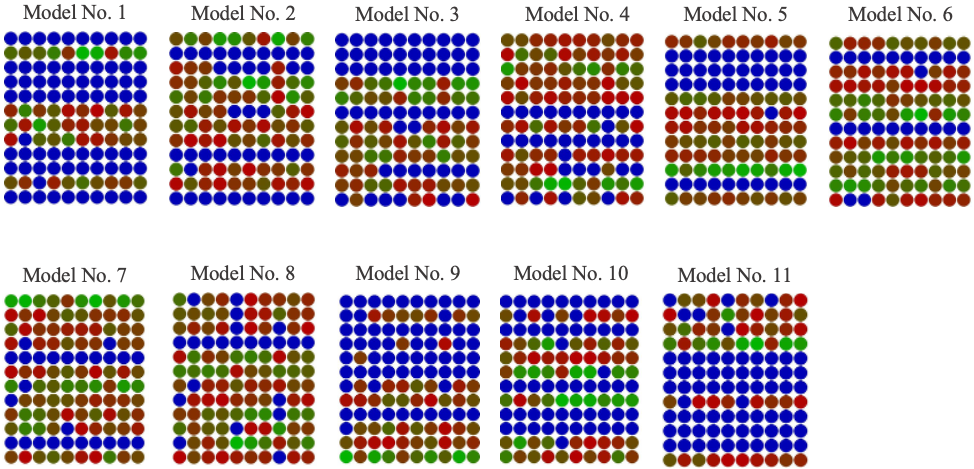
\includegraphics[width=0.99\textwidth]{pre_study_activations}
    \caption[Network activations of classification networks on the straight line dataset]{The activations of the first fully connected layer in the ``head'' of the different networks. For each model, the activity of the $12$ neurons is shown for each class (activations along the vertical axis, classes along the horizontal axis). Red means low activation, green means high activation, blue means activation is off (i.e. $0$).}
    \figlbl{pre_study_activations}
\end{figure}

%It can also be observed that roughly the same neurons are always active.
%For different classes, however, these neurons do not switch on or off, but the strength of the activity changes.

\figref{pre_study_inputs_max} visualizes the input that maximizes the probability for each class.
It is obvious that all models focus on the wrong features and it can be assumed that these networks would not be robust to slight perturbations in the input.
This also indicates that net fragments are not present in current deep learning models (or at least not to the desirable extent);
if a class-level net fragment is composed of several lower-level net fragments, then some of these lower-level net fragments have to be active.
Since these lower-level net fragments represent specific input features, corresponding pixel constellations should be visible in this visualisation.
However, since these rather random-looking pixel combinations maximise the probability of predicting a specific class, this suggests that pixel combinations are not composed into hierarchically more complex net fragments.

\begin{figure}[h]
    \centering
    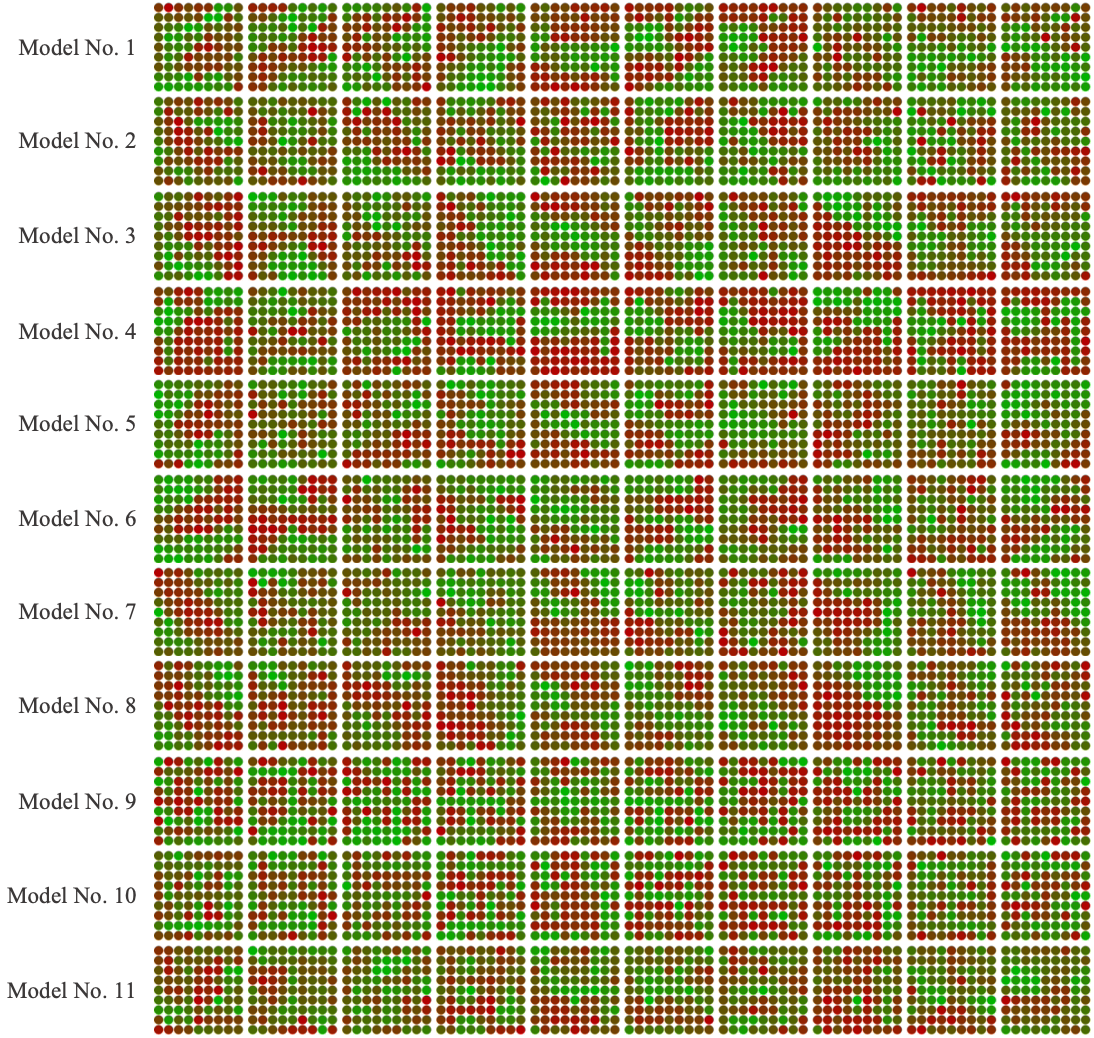
\includegraphics[width=0.99\textwidth]{pre_study_inputs_max}
    \caption[Inputs that Maximize the Class Output Probability]{The inputs that maximize the probability that the different models predict a specific class. For example, the image in the top left corner maximizes the probability that model number $1$ predicts that this is class $0$ (digit $0$).}
    \figlbl{pre_study_inputs_max}
\end{figure}




\section{Autoencoders}\seclbl{pre_study_ae}

\subsection{Methods}\seclbl{pre_study_ae_methods}
Similar to the experiments with classification networks, different autoencoders are also investigated.
Since most architectures lead to similar results for the classification networks, the focus is less on testing many different architectures but rather on incorporating different constraints that might encourage net-fragments.
Incorporating constraints into an autoencoder can be done easily by adding a loss function that regulate the activations in the bottleneck layer.
For a classification network, on the other hand, it is not obvious how such constraints should be added.
The two different autoencoder architectures used are shown in Table  \tabref*{pre_study_ae_models}.

\begin{table}[h]
\newcolumntype{L}[1]{>{\raggedright\let\newline\\\arraybackslash\hspace{0pt}}m{#1}}
\newcolumntype{C}[1]{>{\centering\let\newline\\\arraybackslash\hspace{0pt}}m{#1}}
\newcolumntype{R}[1]{>{\raggedleft\let\newline\\\arraybackslash\hspace{0pt}}m{#1}}
    \tablbl{pre_study_ae_models}
    \centering
	 \begin{tabular}{|l L{9cm}|} 
    	\hline
    	\textbf{No.} & \textbf{Encoder Description} \\
        \hline
		1 & FC (in size=$9*9$ out size=$12$) $\rightarrow$ ReLU $\rightarrow$ FC (in size=$12$ out size=$9*9$) \\ \hline
		2 & FC (in size=$9*9$ out size=$40$) $\rightarrow$ ReLU $\rightarrow$ FC (in size=$40$ out size=$9*9$) \\ \hline
        \hline
    \end{tabular}
    \caption[Different architectures of autoencoders that are investigated for net-fragments]{A description of the different autoencoder networks that are investigated for net-fragments.}
\end{table}


The autoencoder's parameters are optimised by minimising a reconstruction loss (i.e. a distance measurement between the input and the reconstructed output) with the Adam optimizer \sidecite{Kingma2015AdamAM} so that the output looks similar to the input even tough the networks capacity is reduced by a bottleneck-layer in the middle.
The learning rate is $5 \cdot 10^{-4}$, the mini-batch size is $32$ samples and the model is trained for a total of $10$ epochs.

The reconstruction loss $L_{rec}$ used for the different experiments is either the L1 distance (mean absolute error) or the L2 distance (mean square error). If $\boldsymbol{x}$ is the input data with $N$ pixels and $\hat{\boldsymbol{x}}$ is the reconstructed data, then the reconstruction loss can be written as follows:

\begin{equation}\eqlbl{ae_recon}
		L_{rec}(\boldsymbol{x}, \hat{\boldsymbol{x}}) = \begin{cases}
      		\frac{1}{N} \sum^{N}_{n=1}|x_n - \hat{x}_n|, & \text{if use L1 distance}\\
      		\frac{1}{N} \sum^{N}_{n=1} (x_n - \hat{x}_n)^2, & \text{if use L2 distance}
    	\end{cases}
\end{equation}

% https://debuggercafe.com/sparse-autoencoders-using-kl-divergence-with-pytorch/

Optionally, a sparsity and a diversity loss were added to the reconstruction loss to encourage net-fragments.
Since specific neurons of a net-fragment represent certain features, they should only be active if the feature is present.
Good features only occur as part of a few objects and not in all of them: Thus, the neurons representing this feature should be active only sporadically and therefore the activations should be sparse and diverse.
This combination of sparsity and diversity is also in line with the ideas of LeCun to obtain autonomous machine intelligence \sidecite{LeCun_AMI}.


For the sparsity loss $L_{s}$ the kullback-leibler (KL) divergence is used \sidecite{10-5555-3042573-3042641}.
The hidden representations $\boldsymbol{z}$ in the bottleneck layer with length $m$ (i.e. $m$ neurons in the bottleneck layer) are defined as $\boldsymbol{z} = z_1, ..., z_m$.
Furthermore, the average activation probability of a neuron $z_j$ over the input data $\boldsymbol{x}$ can be calculated as

\begin{equation}\eqlbl{ae_kldd}
		\hat{\rho}_j = \frac{1}{N} \sum^N_i \frac{1}{1+e^{-z^{(l)}_i}}
\end{equation}

where $\frac{1}{1+e^{-z^{(i)}}}$ is the sigmoid function that squeezes the activation in the range between $0$ and $1$. Furthermore, $\rho=0.05$ is sparsity parameter that can be interpreted as a target activation probability of each neuron. If the kullback-leibler divergence between all $\hat{\rho}_j$ and $\rho$ is minimised, then an average activation probability per neuron in the hidden layer of $\rho$ is enforced. The corresponding kullback-leibler divergence for each $\hat{\rho}_j$ is defined as:


\begin{equation}\eqlbl{ae_kld}
		KL(\rho || \hat{\rho}_j) = \rho \cdot \log \frac{\rho}{\hat{\rho}_j} + (1-\rho) \cdot \log \frac{1-\rho}{1-\hat{\rho}_j}
\end{equation}

The sparsity loss $L_{s}$ is the sum of the kullback-leibler divergence between all $\hat{\rho}_j$ and $\rho$ and thus enforces that on average only $5\%$ of the hidden representations $\boldsymbol{z}$ are active:

\begin{equation}\eqlbl{ae_kldl}
		L_{s}(\rho, \hat{\rho}) = \sum_{j=1}^{m} KL(\rho || \hat{\rho}_j)
\end{equation}

Thus, this constraint ensures that the activations are sparse, which is consistent with the concept of net-fragments.
Another property of net-fragments is that the activations should be diverse.
Therefore, a new diversity loss $L_{d}$ is proposed.
This loss is based on the fact that the activations in the bottleneck layers $(\boldsymbol{z}^{(1)}, ..., \boldsymbol{z}^{(N)})$ should be as different as possible for all samples of a mini-batch $(\boldsymbol{x}^{(1)}, ..., \boldsymbol{x}^{(N)})$.
It is easy to see that the sum of the dot product between the activation of a sample $\boldsymbol{z}^{(i)}$ and all other samples $\boldsymbol{z}^{(j)}$, $i \neq j$ is small if the samples within a batch have a high diversity. Therefore, the diversity loss can be defined as:

\begin{equation}\eqlbl{ae_kldl2}
		L_{d}(\boldsymbol{z}) = \frac{1}{N} \sum_{i=1}^N\sum_{j=1}^{m} \boldsymbol{z}^{(i)} \cdot \boldsymbol{z}^{(j)}, \text{ if } i\neq j
\end{equation}

Minimising $L_{d}$ results in the bottleneck layer activations not only being sparse but also diverse. 
The overall loss can be defined as the sum of these three loss components, with $\lambda_s$ and $\lambda_d$ beeing hyperparameters that control the influence of the diversity and sparsity loss.

\begin{equation}\eqlbl{ae_kldl2}
		L = L_{rec} + \lambda_s \cdot L_{s} + \lambda_d \cdot L_{d}
\end{equation}

In the experiments, these hyperparameters were set to $\lambda_s = 0.02$ and $\lambda_d = 0.02$, respectively $\lambda_s = 0$ and $\lambda_d = 0$ if the sparsity and diversity loss should not be used.

Similar to the analysis of classification architectures, the model's activations of each layer are stored after every epoch.
These vectors are visualized and investigated for net fragments.

\subsection{Results}\seclbl{pre_study_ae_results}
The activations of the autoencoders trained with reconstruction loss only and without diversity or sparsity constraint (i.e. $\lambda_s = 0$ and $\lambda_d = 0$) look very similar to those of the classification network; about half of the neurons are always active regardless of the object depicted in the image and the other half of neurons are always inactive. Thus, this version of the autoencoder has the same problem as the classification networks. Adding a sparsity constraint (i.e. $\lambda_s = 0.02$ and $\lambda_d = 0$) improves this issue slightly. The activations become sparse, but the same neurons are always active independent of the objects in the image. Only in a few cases can a set of neurons be identified that represent specific objects or features.

However, if all three loss components are used, the activations look much better. In this case, specific neuron combinations represent object-dependent features and are only active for specific objects. There are no more neurons that are constantly active. It is even possible to infer image labels based on a binary activity state (i.e. which neuron is active or inactive) and without knowing the strength of the activation, even though labels were not used during training. Thus, an autoencoder with additional sparsity and diversity constraint can represent net-fragments to some extent\sidenote{except that constraint 1 which says that net-fragments span several layers by design is violated (c.f. Introduction in Section \secref*{net_fragments})}.


\begin{figure}[h]
    \centering
    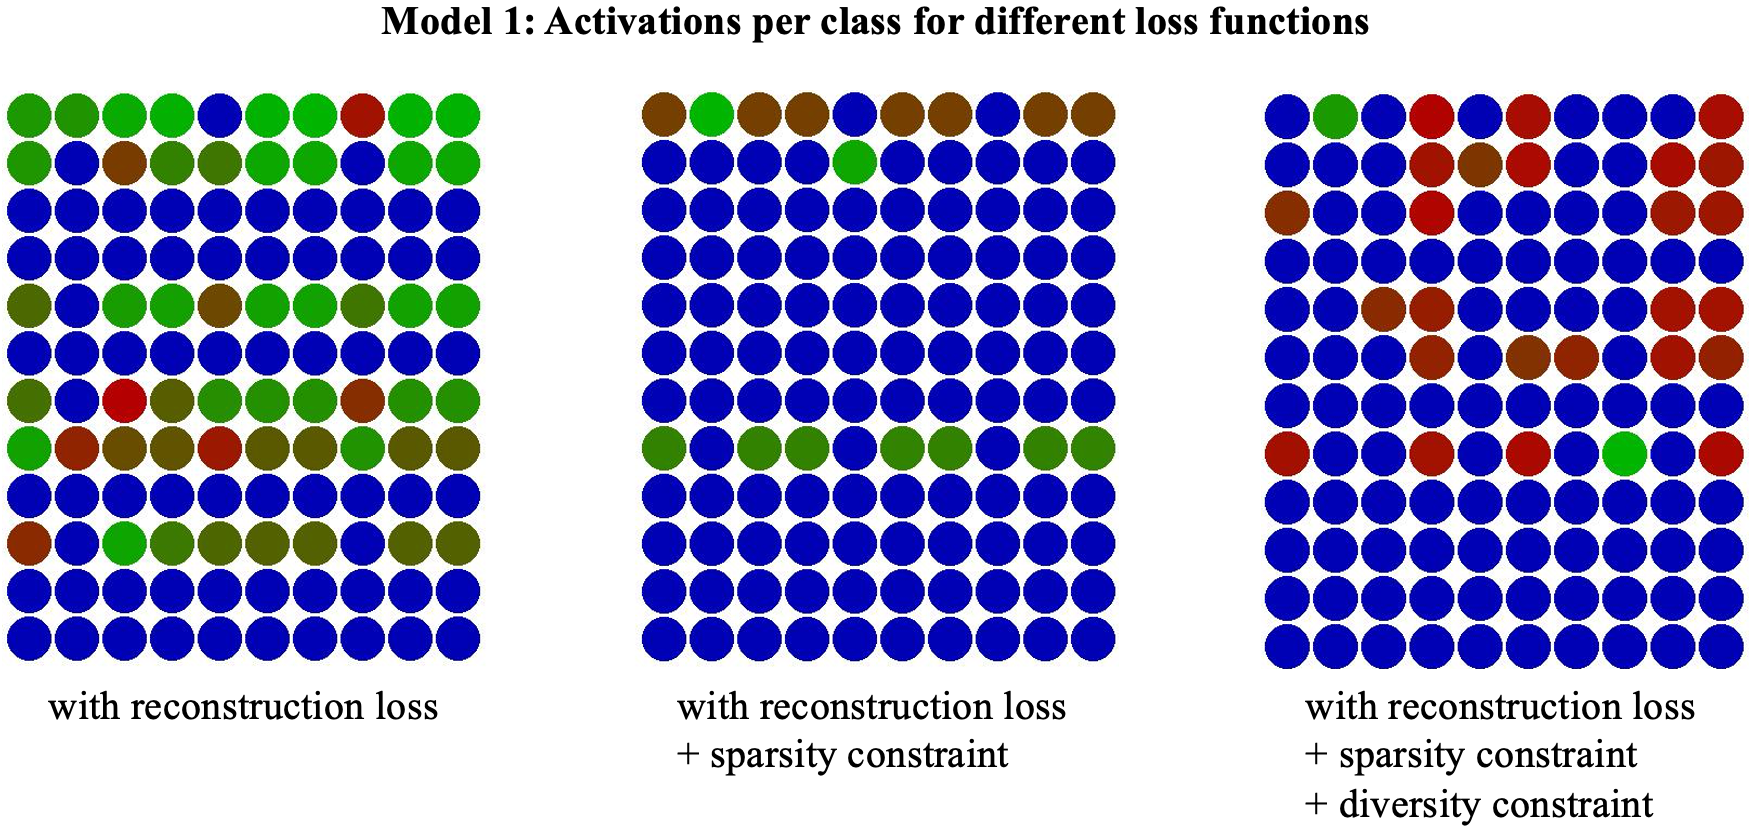
\includegraphics[width=0.99\textwidth]{pre_study_ae1}
    \caption[Network activations of the smaller autoencoder network on the straight line dataset]{The activations in the bottleneck layer of the smaller autoencoder ``model 1'' for different loss functions. For each loss function, the activity of the $12$ neurons in the bottleneck layer is shown for each class (activations along the vertical axis, classes along the horizontal axis). Red means low activation, green means high activation, blue means activation is off (i.e. $0$).}
    \figlbl{pre_study_ae1}
\end{figure}


This can be observed in Figure \figref*{pre_study_ae1} that shows the activations of the ``model 1''.
On the left are the activations without constraint, in the middle the activations with sparsity constraint and on the right the activations with sparsity and diversity constraint.
For each of these three loss functions, the activations in the bottleneck layer are shown per class (activations along the vertical axis, classes along the horizontal axis).
It is clearly visible how adding the sparsity constraint and the diversity constraint gives more meaning to the individual neurons. While without both constraints the same neurons are always active independent of the class, the activations are significantly more varied when both constraints are used.
This becomes even more obvious when the activations of the bigger autoencoder ``model 2'' are investigated (c.f. Figure \figref*{pre_study_ae2} (a)).

\begin{figure}[h]
    \centering
    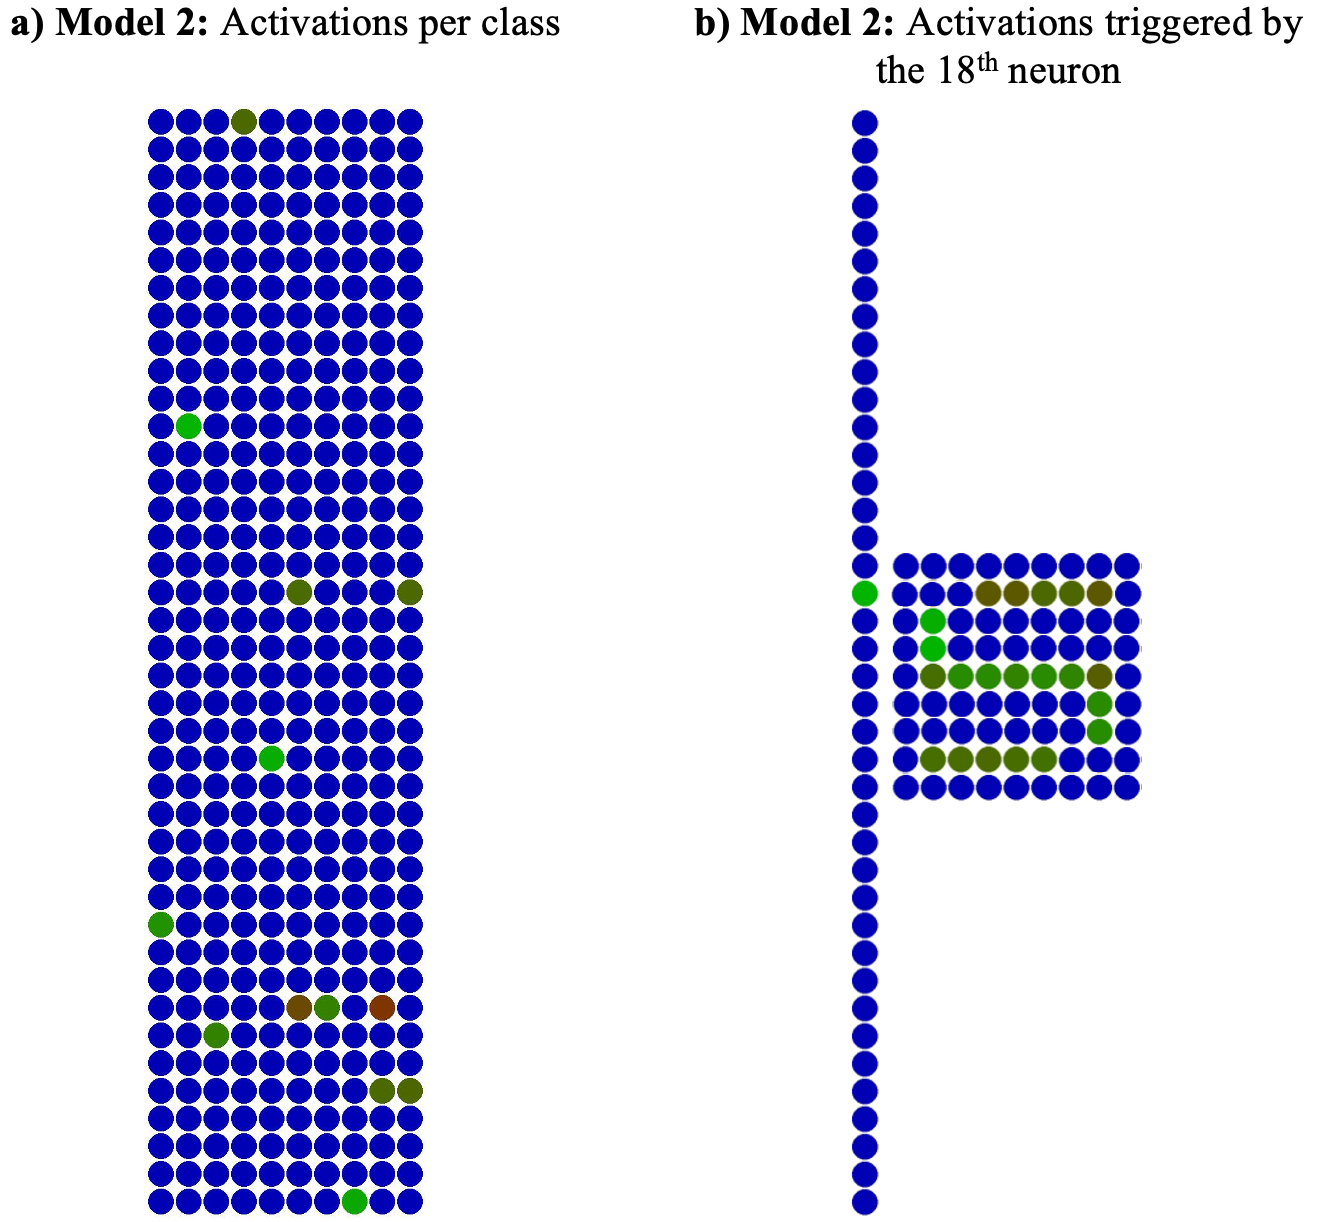
\includegraphics[width=0.99\textwidth]{pre_study_ae2}
    \caption[Network activations of the bigger autoencoder network on the straight line dataset]{On the lieft sinde (a), the activations in the bottleneck layer of the bigger autoencoder ``model 2'' are shown. The activity of the $40$ neurons in the bottleneck layer is shown for each class (activations along the vertical axis, classes along the horizontal axis). On the right side (b), the output of the decoder is shown when the 18th neuron is set to $1$ and all other neurons are set to $0$. The $18$-th neurons is a feature that is needed to generate the numbers $5$ and $9$.}
    \figlbl{pre_study_ae2}
\end{figure}

It is also examined what features the various neurons in the bottleneck layer represent.
This is done by manually creating a bottleneck activation $\boldsymbol{z} = z_1, ..., z_m$ and feeding it through the decoder.
To examine which feature the $i$-th neuron represents, $z_i=1$ is set and $z_{j}=0$, for $i \neq j$.
Figure \figref*{pre_study_ae2} (b) shows which feature the $18$-th neuron represents. Together with the $33$-th neuron, this neuron represents the number 5 and together with the $36$-th neuron the number 9.
Thus, it is a feature (i.e. a net-fragment) that assembles with other features to represent an object.


\section{Conclusion}\seclbl{pre_study_conclusion}
Different architectures have been trained with different targets on a very simple and therefore easily interpretable data set.
The network activations are tracked during training and analyzed for net-fragments.
Typical vision architectures are sequential and build up a composition of features (i.e. net-fragments) over several layer.
Usually, the embeddings of a pre-defined layer are used for down-stream tasks such as classification.
Autoencoders typically use the bottleneck layer, a classification networks typically have a classification head (i.e. a FC layer with a Softmax activation) after the last model layer and thus extract these embeddings from the last model layer.
Thus, embeddings are extracted from one layer.
Net-fragments, on the other hand, span over multiple layers\sidenote{net-fragments can be thought of as the ``path'' of features through a network} and hence this principle is violated.

Furthermore, net fragments are strongly active when the corresponding feature they represent is present in the input and are weakly active or not active at all when it is not present.
Typical deep learning networks have neurons that are never active, while the active neurons usually remain active regardless of the class of the input data and only change their activity slightly.
Thus, the information about different features is not distributed on different neurons but transported as activation strength of neurons through the network.
Therefore, deep learning architectures do not comprise brain-like net fragments by default.

However, it was found that adding a sparsity and diversity constraint can alleviate this issue.
Adding such constraints to the loss function encourages neurons to represent specific features that are typical for some of the objects.
